\documentclass[12pt]{article}
\usepackage{amsmath}
\usepackage{graphicx}
\usepackage{listings}
\usepackage{amsfonts}
\usepackage{amssymb}
\usepackage{hyperref}
\usepackage{tocloft}
\usepackage{multirow}

% \documentclass[tikz,border=10pt]{standalone}
\usepackage{tikz}
\usetikzlibrary{automata, positioning, arrows}

\usepackage[framed,autolinebreaks,useliterate]{mcode}

\title{Problem Sheet 2 Answer}
\author{Junbiao Li - 209050796}
\date{\today}

\renewcommand{\cftsecleader}{\cftdotfill{\cftdotsep}}
% 对于 \section
\renewcommand{\cftsubsecleader}{\cftdotfill{\cftdotsep}}
% 对于 \subsection

\begin{document}

\maketitle
\tableofcontents

\clearpage
\section{Problem 1}

\subsection*{a. Verify that $f$ is a flow and compute its value}

We have \(f(e) \leq w(e)  \forall e \in E\) and
\[
    |f| = 4+0+1 = 5 = 4+1
\]

Hence it is satified the capacity constraint and the flow conservation
constraint.

\subsection*{b. Identify an $f$-augmenting path and compute its capacity.}

We can calculate the capacity of the path \(p = \{S, B, D, T\}\) by
\[
    \varepsilon(p):=\min _{1 \leq i \leq \# p-1}\left\{\begin{array}{cc}
        w\left(p_i, p_{i+1}\right)-f\left(p_i, p_{i+1}\right) & \text { if
        }\left(p_i, p_{i+1}\right) \in E
        \\
        f\left(p_{i+1}, p_i\right)                            & \text {
            otherwise }
    \end{array}\right.
\]

which is
\[
    \epsilon(p) = min \{7-4, 3-1, 6-4 \} = 2
\]

\subsection*{c. Provide a nontrivial upper bound for the value of a maximal
    flow.}

We know that for any flow \(f\) and any s-t cut \(K\), it holds \(|f| \leq c(N, K)\).

We can find that \(K=\{S, A, B\}\) and \(\bar{K}=\{C, D, T\}\), which means \(C(N, K)=4+3+3+3=13\)
Hence the nontrivial upper bound for the value of a maximal flow is \(13\)

The maximum flow of the directed network calculated by MATLAB is 7. Shown in
Figure \ref{fig:og}. MATLAB Code is shown in Appendix \ref{lst:1c}.

\begin{figure}[h]
    \centering
    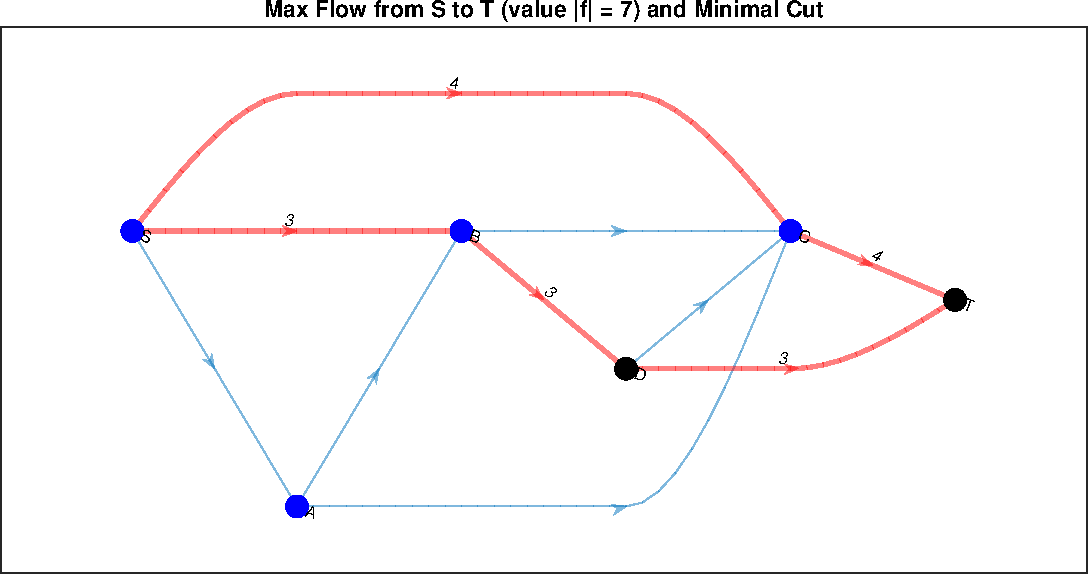
\includegraphics[width=0.6\textwidth]{imgs/mf.pdf}
    \caption{Max Flow From $S$ to $T$}
    \label{fig:og}
\end{figure}

\section{Problem 2}

\subsection*{a. Prim's algorithm Step by Step}

Using Prim's algorithm, we can find the minimal spanning tree of the graph step
by step. Shown in Figure \ref{fig:pm}.

Step 1:

\[
    \begin{aligned}
         & K_0=\{O\}, E_0^{\prime}=\varnothing                       \\
         & C(N, K_0) = \{(O, A), (O, B), (O, C)\}                    \\
         & (O, B) \in \operatorname{argmin}\{w(e): e \in C(N, K_0)\}
    \end{aligned}
\]

Step 2:

\[
    \begin{aligned}
         & K_1=\{O, B\}, E_1^{\prime}=\{(O, B)\}                          \\
         & C(N, K_1) = \{(O, A), (O, C), (B, A), (B, C), (B, D), (B, E)\} \\
         & (B, D) \in \operatorname{argmin}\{w(e): e \in C(N, K_1)\}
    \end{aligned}
\]

Step 3:

\[
    \begin{aligned}
         & K_2=\{O, B, A\}, E_2^{\prime}=\{(O, B), (B, D)\}          \\
         & C(N, K_2) = \{(O, A), (O, C), (B, A), (B, C), (B, E), (D, E), (C, A)\}    \\
         & (D, E) \in \operatorname{argmin}\{w(e): e \in C(N, K_2)\}
    \end{aligned}
\]

Step 4:

\[
    \begin{aligned}
         & K_3=\{O, B, A, C\}, E_3^{\prime}=\{(O, B), (B, D), (D, E)\} \\
         & C(N, K_3) = \{(O, A), (O, C), (B, A), (B, C), (B, E), (D, A), (C, E), (E, T)\}              \\
         & (C, E) \in \operatorname{argmin}\{w(e): e \in C(N, K_3)\}
    \end{aligned}
\]

Step 5:

\[
    \begin{aligned}
         & K_4=\{O, B, A, C, D\}, E_4^{\prime}=\{(O, B), (B, D), (D, E), (C, E)\}                                                                 \\
         & C(N, K_4) = \{(B, A), (D, A), (O, A), (C, T), (E, T)\}
        \\
         & (B, A) \in \operatorname{argmin}\{w(e): e \in C(N, K_4)\}
    \end{aligned}
\]

Step 6:

\[
    \begin{aligned}
         & K_5=\{O, B, A, C, D, E\}, E_5^{\prime}=\{(O, B), (B, D), (D, E), (C, E), (B, A)\}
        \\
         & C(N, K_5) = \{(E, T), (C, T)\}
        \\
         & (E, T) \in \operatorname{argmin}\{w(e): e \in C(N, K_5)\}
    \end{aligned}
\]

\begin{figure}[h]
    \centering
    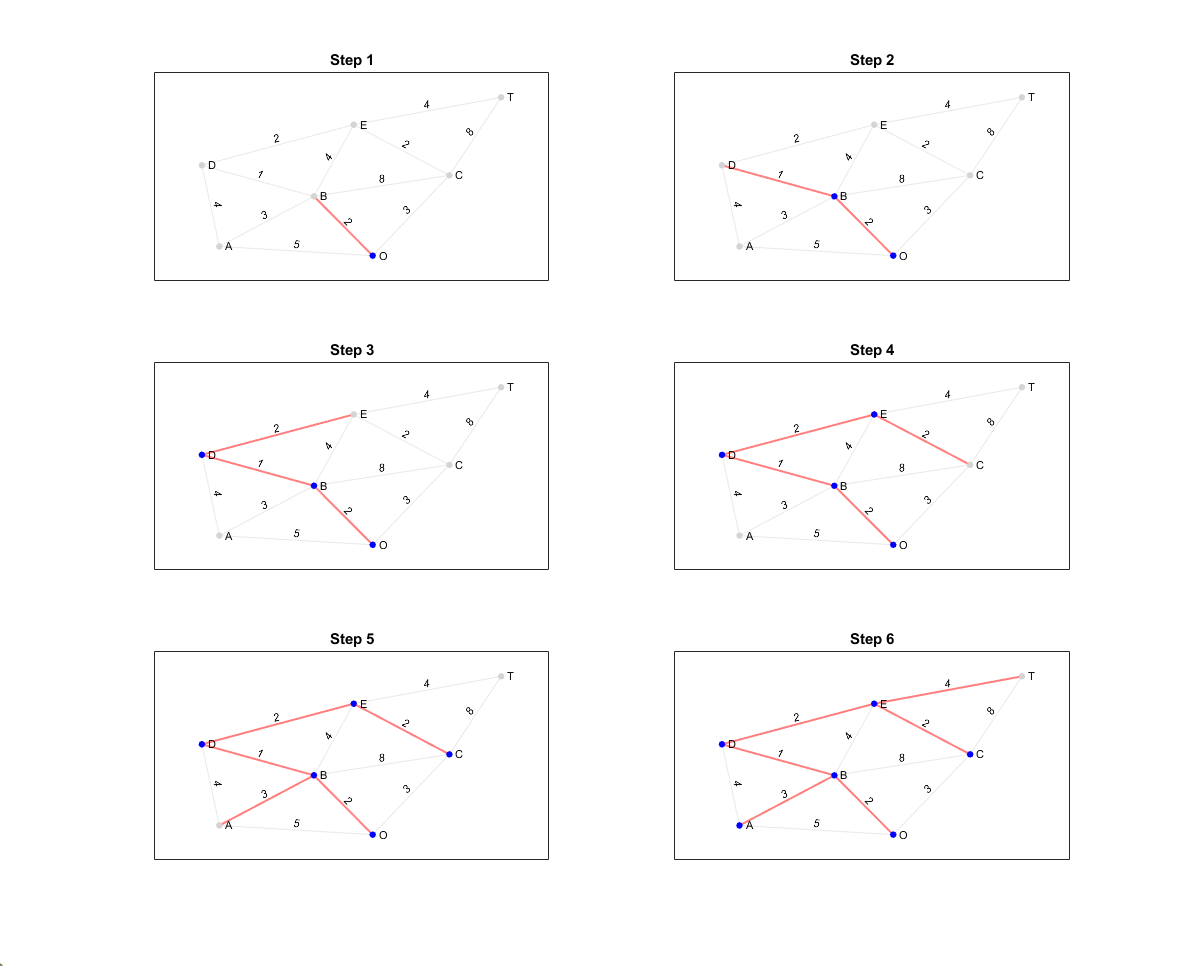
\includegraphics[width=1.\textwidth]{imgs/prim.png}
    \caption{Minimal Spanning Tree Step by Step. The drawing code is displayed in the Appendix \ref{lst:2a}}
    \label{fig:pm}
\end{figure}

\subsection*{b. The Minimal Spanning Tree of the Full Subgraph}

We can find the Minimal Spanning Tree by solving the following linear
programming
\[
    \min \sum_{e \in E} w(e) x_e \text { s.t. }\left\{\begin{array}{c}
        \sum_{e \in E} x_e=|V|-1                                   \\
        \sum_{e \in E^{\prime}} x_e \leq\left|V^{\prime}\right|-1 \quad \forall
        \text { full subgraph }\left(V^{\prime}, E^{\prime}\right) \\
        x_e \in\{0,1\} \forall e \in E
    \end{array}\right.
\]

\begin{enumerate}

    \item \textbf{Objective Function}: \(\min \sum_{e \in E} w(e) x_e\)

          In the MATLAB code, \verb|f = edges(:, 3);| represents the weights of
          the edges
          as coefficients of the objective function.

    \item \textbf{Equality Constraint}: \(\sum_{e \in E} x_e = |V| - 1\)

          In the MATLAB code,
          \verb|Aeq = ones(1, num_edges);beq = num_nodes - 1;| sets
          up this constraint.

    \item \textbf{Inequality Constraint}: \(\sum_{e \in E^{\prime}} x_e \leq
          |V^{\prime}| - 1 \quad \forall \text{ full subgraph } (V^{\prime},
          E^{\prime})\)

          This constraint is the subtour elimination constraint. In the MATLAB
          code, this
          is implemented by iterating over all subsets of vertices and adding a
          constraint for each subset: the \verb|for k = 2:num_nodes-1 ... end|
          loop and
          the subsequent \verb|if all(ismember(edges(j, 1:2), combn(i, :)))|
          condition.

    \item \textbf{Variable Range}: \(x_e \in \{0,1\} \forall e \in E\)

          In the MATLAB code, this is ensured by the integer constraint in the
          \verb|intlinprog| function: \verb|intcon = 1:num_edges;|.

\end{enumerate}

The complete MATLAB Code is shown in Appendix \ref{lst:2b}. The answer is

\begin{lstlisting}
    % Selected edges for the minimal spanning tree:
    % Edge : O-B
    % Edge : O-C
    % Edge : A-B
\end{lstlisting}

\section{Problem 3}

\subsection*{a. Determine the Best Strategies and Explain Why This Game is not
    Stable}

We observe that \(A^{-} = -1 < 2 = A^{+}\) from table \ref{table:a}, therefore
this game is not stable.
Since taht players do not employ mixed-strategies, the best strategies for
player 1 is strategies 1 and strategies 3. The best strategies for player 2 is
strategies 3 and strategies 4.

\begin{table}[]
    \begin{tabular}{|cl|lllll|}
        \hline
        \multicolumn{2}{|l|}{\multirow{2}{*}{A}}        &
        \multicolumn{5}{c|}{Player 2}
        \\ \cline{3-7}
        \multicolumn{2}{|l|}{}                          &
        \multicolumn{1}{l|}{Strategy 1}                 &
        \multicolumn{1}{l|}{Strategy 2}                 &
        \multicolumn{1}{l|}{Strategy 3}                 &
        \multicolumn{1}{l|}{Strategy 4}                 & Min        \\
        \hline
        \multicolumn{1}{|c|}{\multirow{5}{*}{Player 1}} & Strategy 1
                                                        &
        \multicolumn{1}{l|}{0}                          &
        \multicolumn{1}{l|}{2}                          &
        \multicolumn{1}{l|}{1}                          &
        \multicolumn{1}{l|}{-1}                         & -1         \\
        \cline{2-7}
        \multicolumn{1}{|c|}{}                          & Strategy 2
                                                        &
        \multicolumn{1}{l|}{3}                          &
        \multicolumn{1}{l|}{4}                          &
        \multicolumn{1}{l|}{0}                          &
        \multicolumn{1}{l|}{-5}                         & -5         \\
        \cline{2-7}
        \multicolumn{1}{|c|}{}                          & Strategy 3
                                                        &
        \multicolumn{1}{l|}{-1}                         &
        \multicolumn{1}{l|}{3}                          &
        \multicolumn{1}{l|}{0}                          &
        \multicolumn{1}{l|}{2}                          & -1         \\
        \cline{2-7}
        \multicolumn{1}{|c|}{}                          & Strategy 4
                                                        &
        \multicolumn{1}{l|}{-2}                         &
        \multicolumn{1}{l|}{-1}                         &
        \multicolumn{1}{l|}{2}                          &
        \multicolumn{1}{l|}{1}                          & -2         \\
        \cline{2-7}
        \multicolumn{1}{|c|}{}                          & Max
                                                        &
        \multicolumn{1}{l|}{3}                          &
        \multicolumn{1}{l|}{4}                          &
        \multicolumn{1}{l|}{2}                          &
        \multicolumn{1}{l|}{2}                          &            \\
        \hline
    \end{tabular}
    \label{table:a}
\end{table}

\subsection*{b. Determine the Optimal Mixed-Strategy for Player 1.}

An optimal strategy $x^*$ for player 1 solves the linear programming problem

\[
    \begin{aligned}
        \max          & \ v                                               \\
        \text{ s.t. } & \left\{\begin{array}{c}
                                   A^T x \geq(v, \ldots, v)^T \\
                                   (1, \ldots, 1) x=1         \\
                                   x \geq 0, v \in \mathbb{R}
                               \end{array}\right.
    \end{aligned}
\]

After solving this linear programming problem using MATLAB, which shown in the Appendix \ref{lst:3b}, we get The optimal
mixed strategy for player 1 is:

\[
    x = (0.0625, 0.2500, 0.6875, 0)\ \text{and}\ v=0.0625
\]

\section{Problem 4}

\subsection*{a. Expected Value and The Variance of Exponential Distribution
    with Parameter \(\alpha=1\)}

For the Exponential Distribution, we have:

\[
    \begin{aligned}
        \mathbb{E}\left[T\right] & = \alpha^{-1} = 1 \\
        \mathbb{V}\left[T\right] & = \alpha^{-2} = 1
    \end{aligned}
\]

\subsection*{b. }

Since \(V\) and \(W\) are i.i.d, We have

\[
    P[1 \leq T \leq 3 \mid V \leq 3] = \frac{P\left[1\leq T \leq 3\right] \cdot
        P\left[V \leq 3\right]}{P\left[V \leq 3\right]} = P\left[1\leq T \leq
        3\right]
    = 0.318
\]

and by the property of exponential distribution which is
\[
    P\left[T_1+T_2+\cdots+T_{n+1} \leq x\right]=1-\sum_{k=0}^n \frac{(\alpha
        x)^k \exp (-\alpha x)}{k !}
\]

we have
\[
    P[T + V + W \leq 1] = 1 - \left( \frac{1^0 e^{-1}}{0!} + \frac{1^1
        e^{-1}}{1!} + \frac{1^2 e^{-1}}{2!} \right) = 0.0803
\]

\section{Problem 5}

\subsection*{a.}

For the M/M/s/K model, we have

\[
    \lambda_0=\lambda_1=\cdots=\lambda_{K-1}=: \lambda \text { and }
    \lambda_n=0 \text { for } n \geq K
\]

and

\[
    \mu_n=\min (n, s) \mu \text { for } n \geq 1
\]

The sketch to describe this birth-and-death process is shown in
fig.\ref{fig:bd}.

The meaning of the parameters is:
\begin{itemize}
    \item \(\lambda=99\) is the arrival rate: This means an average of \(99\)
          customer arrivals per unit of time
    \item \(\mu=50\) is the service rate: This means that each service desk can
          serve \(50\) customers per unit of time
    \item \(s=2\) is the number of servers: Indicates that there are \(2\)
          service counters that can serve customers at the same time
    \item \(K=100\) is the capacity of the system: Indicates that up to \(100\)
          customers can wait or be served in the system
\end{itemize}

\begin{figure}[htb]
    \centering
    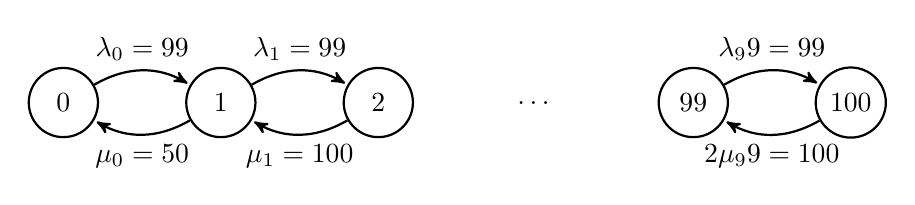
\begin{tikzpicture}[auto, thick, node distance=2cm, >=triangle 45]
        \tikzset{
            % Define standard arrow tip
            >=stealth',
            % Define style for boxes
            punkt/.style={
                    rectangle,
                    rounded corners,
                    draw=black, very thick,
                    text width=6.5em,
                    minimum height=2em,
                    text centered},
            % Define arrow style
            pil/.style={
                    ->,
                    thick,
                    shorten <=2pt,
                    shorten >=2pt,},
        }
        % Draw the states
        \node[state] (s0) {0};
        \node[state, right of=s0] (s1) {1};
        \node[state, right of=s1] (s2) {2};
        \node[draw=none, right of=s2] (sdots) {\ldots};
        \node[state, right of=sdots] (sN1) {99};
        \node[state, right of=sN1] (sN) {100};

        % Connect the states with arrows
        \draw[every loop]
        (s0) edge[bend left, auto=left] node {\(\lambda_0=99\)} (s1)
        (s1) edge[bend left, auto=left] node {\(\mu_0=50\)} (s0)
        (s1) edge[bend left, auto=left] node {\(\lambda_1=99\)} (s2)
        (s2) edge[bend left, auto=left] node {\(\mu_1=100\)} (s1)
        % (s2) edge[bend left, auto=left] node {\ldots} (sdots)
        % (sdots) edge[bend left, auto=left] node {\ldots} (s2)
        % (sdots) edge[bend left, auto=left] node {\ldots} (sN1)
        % (sN1) edge[bend left, auto=left] node {\ldots} (sdots)
        (sN1) edge[bend left, auto=left] node {\(\lambda_99=99\)} (sN)
        (sN) edge[bend left, auto=left] node {\(2\mu_99=100\)} (sN1);

    \end{tikzpicture}
    \caption{Birth-and-Death Process}
    \label{fig:bd}
\end{figure}

\subsection*{b.}

We can calculate \(p_0\) using the following formula:
\[\begin{aligned}
         & \qquad c_n=\frac{\lambda_{n-1} \lambda_{n-2} \ldots \lambda_0}{\mu_n
            \mu_{n-1} \ldots \mu_1}=
        \begin{cases}\frac{1}{n
            !}\left(\frac{\lambda}{\mu}\right)^n &
            \text { for } 0 \leq n \leq s,         \\
            \frac{1}{s

                !}\left(\frac{\lambda}{\mu}\right)^s\left(\frac{\lambda}{s
            \mu}\right)^{n-s}                    &
            \text { for } s \leq n \leq K,         \\
            0                                    &
            \text { for } n>K,\end{cases}         \\
         & \text { and } p_0=\left(1+\sum_{n=1}^{\infty}
        c_n\right)^{-1}=\left(1+\sum_{n=1}^K c_n\right)^{-1}
    \end{aligned}
\]
Solving with MATLAB, which shown in Appendix \ref{lst:5b}, we get \(p_0 = 0.0079\).

\section{Problem 6}

We have 
\[
    c_n=\frac{\lambda_{n-1} \lambda_{n-2} \ldots \lambda_0}{\mu_n \mu_{n-1} \ldots \mu_1}
\]

and
\[
    \lambda_n = \left\{
    \begin{array}{l}
        3 \text { for } n \text { even } \\
        1 \text { for } n \text { odd }
    \end{array}\right.
\]

According to the steady-state condition, since \(\lambda_n \neq 0\ \forall n \) we hvae to make sure that\(\sum c_n \neq \infty \), which means \(\mu \geq 3\) since the series \(c_n\) converge if and only if \(\mu \geq 3\)

\section{Problem 7}

\subsection*{a. Determine all stationary points of \(f\) in \(\mathbb{R}\)}

In order to find the stationary points of \(f\), we need to find the roots of
the derivative of \(f\). We have

\[
    \nabla f(x)=f^{\prime}(x) = 4x^3 - 6x^2 + 2x
\]

Letting \(\nabla f(x)=0\) we have  \(x = 0\), \(x = \frac{1}{2}\), and \(x
= 1\).

\subsection*{b. Perform one step of Newton's method}

Recall that
\[
    \begin{aligned}
        x_{n+1}             &
        =x_n-\frac{f\left(x_n\right)}{f^{\prime}\left(x_n\right)} \\
        \text{Which means } &
        \\
        x_{1}               &
        =x_0-\frac{f\left(x_0\right)}{f^{\prime}\left(x_0\right)} \\
    \end{aligned}
\]

Hence, we have
\[
    x_1 = -1 - \frac{4}{-12} = -0.6667
\]

\subsection*{c. Perform one step of the steepest descent method}

Consider the function \(f(x) = x^4 - 2x^3 + x^2\).

We have
\[ f'(x) = \frac{d}{dx}(x^4 - 2x^3 + x^2) = 4x^3 - 6x^2 + 2x \] and the initial
point is \(x_0 = -1\).

\[ f'(-1) = 4(-1)^3 - 6(-1)^2 + 2(-1) = -12 \]

To find the smallest optimal step size, we set up a new function \(g(\alpha) =
f(x_0 - \alpha \cdot f'(x_0))\) and differentiate it:
\[ g(\alpha) = f(-1 + 12\alpha) \]

We then differentiate \(g(\alpha)\) and solve the equation \(g'(\alpha) =
0\) to find the \(\alpha\) that minimizes \(g(\alpha)\).

We use the found optimal step size \(\alpha\) to calculate the new point
\(x_1\):
\[ x_1 = x_0 - \alpha \cdot f'(x_0) \]

By solving \(g'(\alpha) = 0\), we have \(\alpha = \frac{1}{12}\).

\[ x_1 = -1 - \frac{1}{12} \cdot (-12) = 0 \]

In summary, using the steepest descent method starting from \(x_0 = -1\), we
found the optimal step size \(\alpha = \frac{1}{12}\) and calculated the next
point \(x_1 = 0\). This indicates that on the given function, moving in the
direction of steepest descent with the optimal step size leads us to the point
0.

\section{Problem 8}

Considering the function  \(f(x):=(A x-b)^T(A x-b)\), to perform Newton's
Method we have to calculate the gradian of \(f\) and the Hessian of \(f\).
Which is
\[
    \begin{aligned}
        \nabla f(x) & =2 A^T(A x-b)          \\
        H(f)(x)     & =\nabla^2 f(x)=2 A^T A
    \end{aligned}
\]

Since \(A\) is invertible, we have \(H(f)(x) = 2 A^T A\) is also invertible.
Hence, we have

\[
    x_{n+1} = x_{n} - \left(2 A^T A\right)^{-1} \cdot 2 A^T(A x_n-b) = x_{n} -
    \left(A^T A\right)^{-1} \cdot A^T(A x_n-b)
\]


\section{Problem 9}

Considering that,
\[
    \begin{aligned}
        L(x, u, p)= & f(x, u)-p^T(A(x) u-b)           \\
        =           & u_1+\cos \left(u_2\right) - p^T
        \left(
        \left(\begin{array}{cc}
                  1+x^2 & x \\
                  x     & 1
              \end{array}\right) u - \left(
        \begin{array}{l}
            1 \\
            1
        \end{array}\right)
        \right)
    \end{aligned}
\]

Differentiating \(L(x, u, p)\) with respect to the variable \(p\) gives the
state equation
\[
    \left(\begin{array}{cc}
            1+x^2 & x \\
            x     & 1
        \end{array}\right) u=\left(\begin{array}{l}
            1 \\
            1
        \end{array}\right)
\]

Differentiating \(L(x, u, p)\) with respect to the variable \(u\) gives the
adjoint equation
\[
    \left(1,-\sin \left(u_2\right)\right)^T=\left(\begin{array}{cc}
            1+x^2 & x \\
            x     & 1
        \end{array}\right)^T p
\]

We can get that

\[
    p = \left(\begin{array}{c}
        p_1 \\
        p_2
    \end{array}\right)= \left(\begin{array}{c}
            x \sin \left(u_2\right)+1 \\
            -x^2 \sin \left(u_2\right)-x-\sin \left(u_2\right)
        \end{array}\right)
\]

\[
    u = \left(\begin{array}{c}
        u_1 \\
        u_2
    \end{array}\right)= \left(\begin{array}{c}
            1-x \\
            x^2-x-1
        \end{array}\right)
\]

Hence, we have
    \[
        \begin{aligned}
            \nabla_x L(x, u, p) & = -\nabla_x\left(p^{T}
            \left(
            \begin{array}{cc}
                1+x^2 & x \\
                x     & 1
                \end{array}
            \right) u\right)
            \\
            &=-\nabla_x\left((1+x^2)p_1u_1+xp_2u_1+xp_1u_2 \right)\\
            &=(1-2 x) \sin \left(x^2-x+1\right)-1
        \end{aligned}
\]

\clearpage
\appendix
\section*{Appendix}
\addcontentsline{toc}{section}{Appendix}
\renewcommand{\thesubsection}{\Alph{subsection}}

\subsection{MATLAB Code}

\begin{lstlisting}[label=lst:1c,
    caption=Problem 1.c]
    % Problem 1.c

    clear; close all;

    % S A B C D T
    % 1 2 3 4 5 6
    edges =  [...
        1 2 5;  % S->A
        1 3 7;  % S->B
        1 4 4;  % S->C
        2 3 1;  % A->B
        2 4 3;  % A->C
        3 5 3;  % B->D
        3 4 3;  % B->C
        4 6 4;  % C->T
        5 6 6;  % D->T
        5 4 1]; % D->C
    
    names = {'S', 'A', 'B', 'C', 'D', 'T'};
    G = digraph(edges(:,1), edges(:,2), edges(:,3), names);
    
    figure;
    subplot(2,1,1)
    p = plot(G, 'EdgeLabel', G.Edges.Weight);
    title('Original Network')
    view([-90 90]);
    
    subplot(2,1,2)
    [mf, GF, cs, ct] = maxflow(G, 1, 6);
    H = plot(G, 'EdgeLabel', G.Edges.Weight);
    view([-90 90]);
    H.EdgeLabel = {};
    highlight(H, GF, 'EdgeColor', 'r', 'LineWidth', 2);
    st = GF.Edges.EndNodes;
    labeledge(H, st(:,1), st(:,2), GF.Edges.Weight);
    title(['Max Flow from S to T (value |f| = ' num2str(mf) ') and Minimal Cut'])
    highlight(H, cs, 'NodeColor', 'blue', 'MarkerSize', 10)
    highlight(H, ct, 'NodeColor', 'black', 'MarkerSize', 10)
\end{lstlisting}


\begin{lstlisting}[label=lst:2a,
    caption=Problem 2.a]
    % Problem 2.a
    % O A B C D E T
    % 1 2 3 4 5 6 7 
    % create a matrix with edges: initial node, final node, and weight
    clear; close all;
    
    edges = [
        1 2 5;
        1 3 2;
        1 4 3;
        2 3 3;
        2 5 4;
        3 5 1;
        3 6 4;
        3 4 8;
        4 6 2;
        5 6 2;
        4 7 8;
        6 7 4;
    ];
    
    node_names = {'O', 'A', 'B', 'C', 'D', 'E', 'T'};
    
    G = graph(edges(:,1), edges(:,2), edges(:,3), node_names);
    
    [T, steps, visited] = prims_algorithm(G, 'O');
    
    lightgrey = [0.83, 0.83, 0.83];
    
    figure;
    disp(steps)
    for i = 1:length(steps)
        subplot(3, 2, i);
        H = plot(G, 'EdgeLabel', G.Edges.Weight, 'NodeColor', lightgrey, 'EdgeColor', lightgrey);
        hold on;
        highlight(H, visited(1:i), 'NodeColor', 'b');
        highlight(H, steps{i}.Edges.EndNodes(:,1), steps{i}.Edges.EndNodes(:,2), 'EdgeColor', 'r', 'LineWidth', 1.5);
        title(sprintf('Step %d', i));
        hold off;
    end
    
    % Prim's 
    function [T, steps, visited] = prims_algorithm(G, start_node)
        nodes = G.Nodes.Name;
        T = graph([], [], [], nodes);
        visited = {start_node};
        steps = {};
    
        while length(visited) < numnodes(G)
            min_edge = [];
            min_weight = inf;
    
            for v = visited
                edges = outedges(G, v{1});
                for e = edges'
                    neighbor = setdiff([G.Edges.EndNodes(e, :)], v);
                    if ~ismember(neighbor, visited)
                        weight = G.Edges.Weight(e);
                        if weight < min_weight
                            min_edge = [v, neighbor];
                            min_weight = weight;
                        end
                    end
                end
            end
    
            T = addedge(T, min_edge{1}, min_edge{2}, min_weight);
            visited{end+1} = min_edge{2};
            steps{end+1} = T;
        end
    end
\end{lstlisting}
\begin{lstlisting}[label=lst:2b,
    caption=Problem 2.b]
    % Problem 2.b
    % Expected Output: 
    % Selected edges for the minimal spanning tree:
    % Edge: O-B
    % Edge: O-C
    % Edge: A-B
    
    clear; close all;
    
    % O A B C
    % 1 2 3 4
    % create a matrix with edges: initial node, final node, and weight
    edges = [
        1 2 5;
        1 3 2;
        1 4 3;
        2 3 3;
        3 4 8;
    ];
    
    node_names = {'O', 'A', 'B', 'C'};
    nodes = unique(edges(:, 1:2));
    num_nodes = length(nodes);
    num_edges = size(edges, 1);
    
    f = edges(:, 3);
    
    Aeq = ones(1, num_edges);
    beq = num_nodes - 1;
    
    A = [];
    b = [];
    
    % Inequality Constraint
    for k = 2:num_nodes-1
        combn = nchoosek(nodes, k);
        for i = 1:size(combn, 1)
            constraint = zeros(1, num_edges);
            for j = 1:num_edges
                if all(ismember(edges(j, 1:2), combn(i, :)))
                    constraint(j) = 1;
                end
            end
            A = [A; constraint];
            b = [b; k - 1];
        end
    end
    
    % Variable Range
    lb = zeros(num_edges, 1);
    ub = ones(num_edges, 1);
    
    intcon = 1:num_edges;
    [x, fval] = intlinprog(f, intcon, A, b, Aeq, beq, lb, ub);
    
    disp('Selected edges for the minimal spanning tree:');
    for i = 1:num_edges
        if x(i) == 1
            disp(['Edge: ' node_names{edges(i, 1)} '-' node_names{edges(i, 2)}]);
        end
    end
    
\end{lstlisting}
\begin{lstlisting}[label=lst:3b,
    caption=Problem 3.b]
    % Problem 3.b
    % Excepted Output:
    % Optimal solution found.
    % 
    % Optimal Mixed Strategy for Player 1:
    %     0.0625
    %     0.2500
    %     0.6875
    %          0
    % 
    % Optimal Value:
    %     0.0625
    
    clear; close all;
    
    % Payoff Matrix
    A = [0, 2, 1, -1;
         3, 4, 0, -5;
         -1, 3, 0, 2;
         -2, -1, 2, 1];
    
    c = [1; zeros(4, 1)];
    
    A_ub = [-ones(4, 1), -A']; % A^T x >= v
    b_ub = zeros(4, 1);
    
    A_eq = [0, ones(1, 4)]; 
    b_eq = 1;
    
    lb = [-inf; zeros(4, 1)]; 
    ub = []; 
    
    options = optimoptions('linprog', 'Algorithm', 'dual-simplex');
    [x, fval] = linprog(c, A_ub, b_ub, A_eq, b_eq, lb, ub, options);
    
    optimal_mixed_strategy = x(2:end);
    optimal_value = -fval;
    
    disp('Optimal Mixed Strategy for Player 1:');
    disp(optimal_mixed_strategy);
    disp('Optimal Value:');
    disp(optimal_value);
    
\end{lstlisting}
\begin{lstlisting}[label=lst:5b,
    caption=Problem 5.b]
    % Problem 5.b
    % Excepted Output: 
    % The Probability of p_0 is: 
    %     0.0079
    s = 2;
    K = 100;
    lambda = 99;
    mu = 50;
    
    c = zeros(1, K+1);
    c(1) = 1;  % c_0 is always 1
    for n = 1:s
        c(n+1) = c(n) * lambda / (n * mu);
    end
    for n = s+1:K
        c(n+1) = c(n) * lambda / (s * mu);
    end
    
    p_0 = 1 / sum(c);
    
    disp('The Probability of p_0 is: ');
    disp(p_0);
    
\end{lstlisting}

\end{document}